% !TeX spellcheck = nl_NL
\chapter{Inleiding}

\section{Situering}\label{sec:situering}

Tegenwoordig zijn quadcopters erg populair voor zowel priv\'e als professioneel gebruik. Een belangrijke reden hiervoor is dat ze makkelijk te verkrijgen zijn en ook helemaal niet zo duur. Dit is te wijten aan hun eenvoudig ontwerp: vier armen met elk \'e\'en propeller. Door dit ontwerp is een quadcopter in staat om verticaal op te stijgen en te landen. Een nadeel is wel dat quadcopters van nature erg onstabiel zijn. De kleinste fluctuaties in motorsnelheden kunnen ervoor zorgen dat een quadcopter zijn evenwicht verliest. Om het evenwicht te herstellen moeten de snelheden van de vier motoren worden aangepast. Voor de mens is dit een te complexe taak. Daarom moet er elektronische stabiliteit voorzien worden. Hiervoor is heel wat rekenkracht nodig. Dankzij de ontwikkelingen binnen de electronica van de laatste jaren is dit in tegenstelling tot vroeger wel mogelijk. De besturing van een quadcopter wordt hierdoor erg vereenvoudigd. Een AR.Parrot is zelfs te besturen met een smartphone. Er wordt een Parrot afgebeeld in figuur \ref{fig:parrot}.

\begin{figure}[h]
	\centering
	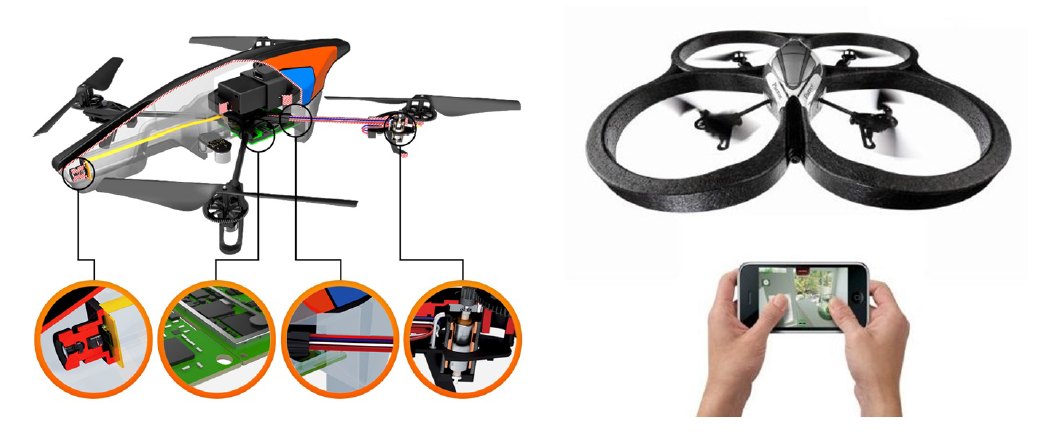
\includegraphics[width=0.6\linewidth]{parrot}
	\caption{AR.Parrot quadcopter drone die met een smartphone bestuurd kan worden.}
	\label{fig:parrot}
\end{figure}

\npar Quadcopters kunnen ingezet worden voor tal van taken. Recent kondigden de `Lokerse Feesten' bijvoorbeeld aan dat ze quadcopters willen inzetten om drank tot bij de festivalgangers te brengen die in de massa staan \cite{url:lokerse}. Uiteraard is dit geen baanbrekend idee. Er werd in het verleden reeds onderzoek gedaan naar quadcopters die in staat zijn om pakketten te leveren \cite{paper:deliveryQuad}.

% drones veiligheidsinspectie
\npar Naast het leveren van pakketten kunnen drones veiligheidsinspecties doen van hoge structuren, die moeilijk te bereiken zijn voor de mens. Hierbij wordt bijvoorbeeld rond een brug gevlogen en wordt de brug gescand op micro-scheurtjes \cite{paper:structureInspection1}\cite{paper:structureInspection2}. Om betrouwbare metingen te kunnen doen, is het belangrijk dat het gebruikte platform niet beweegt tijdens het scannen. Bovendien is het de bedoeling dat de leercurve voor het vliegen met dit platform zo laag mogelijk is. Op manier kan een persoon met weinig vliegervaring het platform toch bedienen. De input van de gebruiker wordt daarom zo laag mogelijk gehouden. Het is natuurlijk ook belangrijk dat het platform niet te pletter vliegt tegen de structuren dat het moet inspecteren. Daarom worden obstakels automatisch ontweken.

% drones mapping
\npar In deze thesis worden drones onderzocht die ingezet kunnen worden voor zogenaamde \textit{search and rescue} missies. Quadcopters zijn hiervoor beter geschikt dan grondrobots omdat ze gemakkelijk over obstakels kunnen vliegen die op de grond liggen \cite{paper:SLAMQuad2}\cite{paper:SearchRescueQuad}. Hier wil men beroep doen op drones om bijvoorbeeld een gevaarlijke site te verkennen en in kaart te brengen. Op die manier zullen reddingswerkers effici\"enter en veiliger te werk kunnen gaan. Voor het genereren van een kaart kan \textit{Simultaneous Localization and Mapping} (SLAM) gebruikt worden. SLAM bleek in het verleden al de beste oplossing voor omgevingsmapping met grondrobots. Het is dan ook niet meer dan logisch dat dezelfde techniek wordt gebruikt voor mapping en exploratie met quadcopters \cite{paper:SLAMQuad}. In \ref{sec:omgmapping} wordt reeds bestaand werk omtrent omgevingsmapping met onbemande vliegende platformen verder belicht.

\subsection{Situering van autonomie bij quadcopters} \label{sec:lcsturing}
Wanneer een quadcopter \'e\'en van de taken beschreven in \ref{sec:situering} autonoom kan uitvoeren, dan wordt het pas echt interessant. Een platform kan als autonoom beschouwd worden van zodra het staat is een taak uit te voeren zonder hulp van buitenaf. Een quadcopterplatform zal maar in staat zijn \'e\'en van de taken in \ref{sec:situering} te vervullen wanneer het stabiel vlieggedrag vertoont. Dit houdt in dat het platform gelijk welke positie in de ruimte kan aannemen en aanhouden. Hiervoor moet het platform zijn huidige positie kunnen meten. Eens gemeten, kan er ook bijgestuurd worden wanneer het platform begint af te wijken of wanneer een nieuwe positie gewenst is. Het meten van de eigen positie wordt in wat volgt \textit{lokalisatie} genoemd.

% figuur van D'Andrea
\npar Als gebruik gemaakt wordt van externe sensoren voor lokalisatie, dan spreekt men van centrale sturing. Centrale sturing voor quadcopters is een domein waar reeds veel onderzoek in verricht is.  Voor binnenshuis toepassingen worden quadcopters vaak voorzien van infrarode LED's terwijl aan het plafond een infraroodcamera gemonteerd wordt om de quadcopters te lokaliseren \cite{paper:flyingInvertedPendulum}. Buitenshuis kan GPS gebruikt worden \cite{paper:deliveryQuad}. Het is zo dat bij centrale sturing, quadcopters taken kunnen uitvoeren zonder dat iemand ze moet besturen, maar ze zijn zeker niet helemaal autonoom, want ze steunen op informatie van externe sensoren. Het belangrijkste en misschien ook wel bekendste onderzoek met quadcopters dat van centrale sturing gebruik maakt, is het werk van Andrea et al. Met behulp van centrale sturing kunnen hun quadcopters allerlei heel complexe taken verwezenlijken. Voorbeelden hiervan zijn het balanceren en doorgeven van een ge\"inverteerde pendulum \cite{paper:flyingInvertedPendulum}, het bouwen van complexe structuren \cite{paper:buildingQuad} en het uitvoeren van acrobatische bewegingen \cite{paper:multiflips}. De quadcopters zijn te zien in actie op figuur \ref{fig:quadAndrea}.

\begin{figure}[h]
	\centering
	\subfigure[Twee quadcopters die elkaar een ge\"inverteerde pendulum doorgeven.]{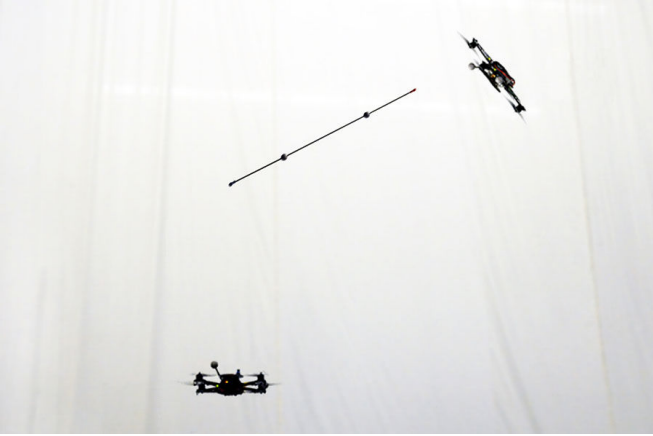
\includegraphics[width=0.48\linewidth, height=6cm]{poleAcrobatics}}
	\hspace{0.01\linewidth}
	\subfigure[Een quadcopter die een touw weeft rond twee andere touwen]{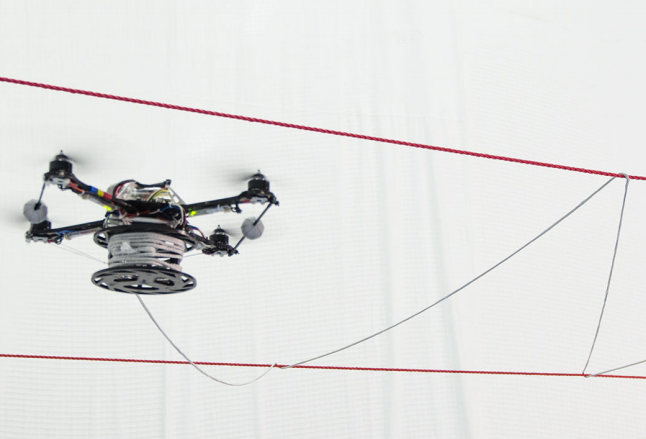
\includegraphics[width=0.48\linewidth, height=6cm]{quadbouwer}} 
	\caption{De quadcopters van Andrea et al. in actie.} \label{fig:quadAndrea}
\end{figure}

\npar Wanneer de quadcopter alle sensoren aan boord heeft, wordt gebruik gemaakt van lokale sturing. Interne sensoren zijn meestal meer onderhevig aan ruis dan externe omdat ze niet veel mogen wegen of in sommige gevallen, zoals in deze thesis, niet veel mogen kosten. Bijgevolg is lokalisatie aan de hand van lokale sturing een stuk moeilijker. In het werk van W. De Gucht wordt optical flow gebruikt, een gelijkaardige aanpak werd reeds eerder onderzocht en heeft zijn kracht bewezen \cite{paper:opticalFlowQuad}. Een andere mogelijkheid is SLAM, deze methode eist echter wel vrij veel rekenkracht. Vaak wordt dan ook een extern toestel gebruikt voor de berekeningen \cite{paper:SLAMQuad}. Het platform kan dan echter niet langer als autonoom beschouwd worden.

\subsection{Omgevingsmapping} \label{sec:omgmapping}
% belangrijkste SLAM implementaties
Binnen alle SLAM implementaties kan men drie groepen onderscheiden. Voor het verzamelen van informatie van de omgeving wordt gebruik gemaakt van ofwel een simpele camera, een laserscanner of een combinatie van die twee. Alle drie de opties hebben hun voor- en nadelen. Een camera biedt heel veel informatie, maar heeft als nadeel dat er niet rechtstreeks diepte uit gehaald kan worden. Laserscanners meten enkel diepte, hun grootste voordeel is dus ook hun grootste beperking. Een combinatie van de twee lijkt dan enkel voordelen te bieden. Dit moet natuurlijk met een korrel zout genomen worden. Het is namelijk niet evident de data van de laserscanner en de camera samen te brengen.

\begin{figure}[h]
	\centering
	\subfigure[Een map gegenereerd met een SLAM algoritme dat een laserscanner gebruikt.]{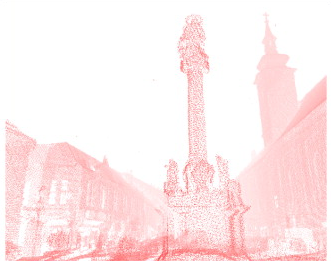
\includegraphics[width=0.45\linewidth]{3DGround2}} \label{fig:3DGrounda}
	\hspace{0.01\linewidth}
	\subfigure[Een map gegenereerd met een SLAM algoritme dat een RGB-D camera gebruikt.]{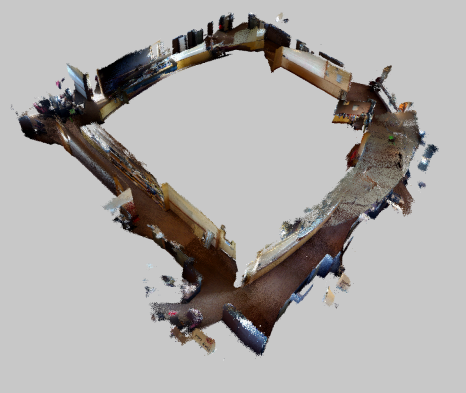
\includegraphics[width=0.45\linewidth]{3DGround}} \label{fig:3DGroundb}
	\caption{Omgevingsmappen gegenereerd door grondrobots met behulp van een 3D laserscanner(a) en met behulp van een RGB-D camera(b).}
\end{figure}

\npar Voor omgevingsmapping met grondrobots is over het algemeen genoeg rekenkracht en geheugen aanwezig om volledige 3D mappen te genereren. Deze zien er dan uit zoals in figuur \ref{fig:3DGrounda}. Om een map te bekomen als deze moet beroep gedaan worden op een vrij dure laserscanner \cite{paper:3DGround2}. Een goedkopere oplossing is een RGB-D camera gebruiken \cite{paper:3DGround}. Dit type camera registreert kleurbeelden en dieptebeelden. In figuur \ref{fig:3DGroundb} wordt een map weergegeven die met dit soort camera werd bekomen.

\npar Wanneer een quadcopter gebruikt wordt, zijn de opties een stuk beperkter. Ten eerste is er de beperkte last die ze kunnen dragen. De gebruikte scanner of camera mag niet te zwaar zijn. Ten tweede beschikt het platform over een beperkte rekenkracht. Het is dan ook zo dat vaak een extern toestel gebruikt wordt voor het genereren van de map. De quadcopter staat dan enkel in voor het verzamelen van de informatie. De thesis van J. Nyman  gebruikt deze aanpak. \textit{Parallel Tracking And Mapping} (PTAM) werd ge\"implementeerd met behulp van een camera \cite{thesis:jens}. Het resultaat is te zien in figuur \ref{fig:PTAM}. In het werk van S. Shen et al. wordt een laserscanner gebruikt in combinatie met een RGB-D camera \cite{paper:3DQuad} . Bovendien gebeuren alle berekeningen aan boord van het platform. Het resultaat is te zien in figuur \ref{fig:3DSlam}. De lezer kan al vermoeden dat de gebruikte hardware voor deze aanpak een heel stuk kostelijker is dan de hardware die J. Nyman gebruikte. Er moet nog opgemerkt worden dat het werk van J. Nyman wel een 3D map genereert, maar die is eigenlijk gebaseerd op 2D data.

%figuur SLAM Jens
\begin{figure}[h]
	\centering
	\subfigure[Een map gegenereerd met de PTAM implementatie van J. Nyman. Het PTAM algoritme maakt gebruik van een camera.]{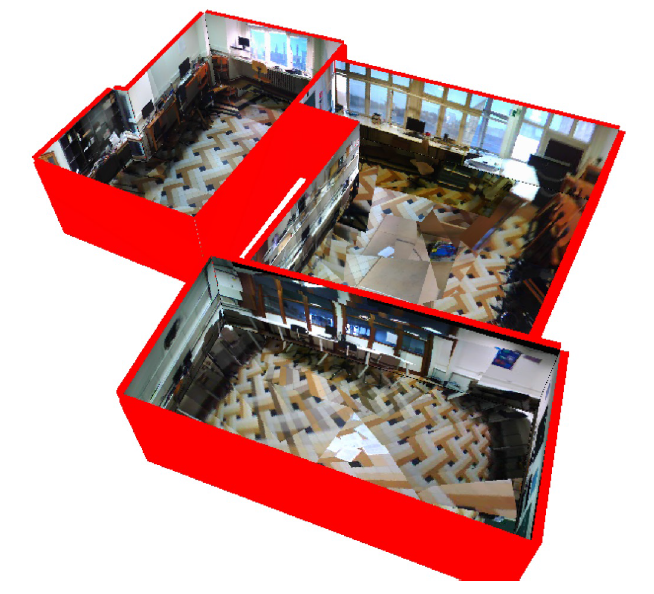
\includegraphics[width=0.45\linewidth]{PTAM}\label{fig:PTAM}}
	\hspace{0.01\linewidth}
	\subfigure[Een map gegenereerd met het SLAM algoritme geschreven door S. Shen et al. dat gebruik maakt van een RGB-D camera en een laserscanner]{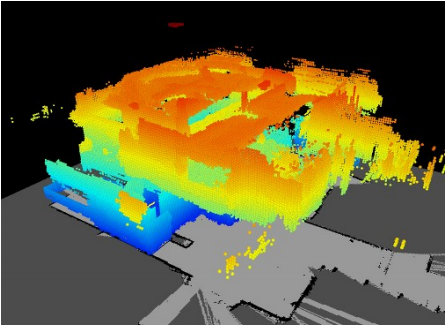
\includegraphics[width=0.45\linewidth]{3DSlam}\label{fig:3DSlam}}
	\caption{Omgevingsmappen gegenereerd door quadcopters met behulp van een camera(a) en met behulp van een laserscanner en een RGB-D camera (b).}
\end{figure}


\section{Probleemstelling}
Er moet een goedkoop \textbf{autonoom platform} gebouwd worden dat zichzelf in evenwicht houdt met behulp van \textbf{lokale sturing}. Dit wil zeggen dat het platform een vaste positie moet kunnen aanhouden zonder weg te driften. Hiervoor mag enkel gebruik gemaakt worden van interne sensoren.

\npar Daarnaast moet het platform geschikt zijn voor \textbf{omgevingsmapping}. Hiervoor moet gebruik gemaakt worden van een laserscanner in combinatie met een SLAM algoritme. Indien nodig kan ook de odometrie van het platform gebruikt worden om een nauwkeurigere omgevingsmap te genereren.

\section{Aanpak}
Om de lezer op de hoogte te brengen van de specificaties en de werking van het platform bij aanvang van deze thesis, wordt hier eerst een hoofdstuk aan besteed. Het is de bedoeling om de quadcopter volledig op zichzelf een onbekende ruimte te laten verkennen. Om geen gevaar te vormen voor zichzelf of voor zijn omgeving, moet het platform voldoende stabiel zijn. Daarom worden in het derde hoofdstuk van deze thesis een aantal optimalisaties voorgesteld om het vlieggedrag van het huidige platform te verbeteren. In hoofdstuk vier wordt er op zoek gegaan naar een geschikt SLAM algoritme om het dan in hoofdstuk vijf te integreren in het platform.
